% -*- coding: utf-8 -*-

\subsection{tf.Variable}

\begin{frame}[fragile]{tf.Variable}
    \begin{tcblisting}{title=RefVariable的读写顺序问题}
        a = tf.Variable(1.0, use_resource=True)
        a.initializer.run()

        assign = a.assign(2.0)
        with tf.control_dependencies([assign]):
          b = a.read_value()
        with tf.control_dependencies([b]):
          other_assign = a.assign(3.0)
        with tf.control_dependencies([other_assign]):
          # Will print 2.0 because the value was read before other_assign ran. If
          # `a` was a tf.Variable instead, 2.0 or 3.0 could be printed.
          tf.Print(b, [b]).eval()
    \end{tcblisting}
\end{frame}

\begin{frame}{主要变动}
    \begin{itemize}
        \item RefVariable: impossible-to-reason-about semantics $\to$ ResourceVariable
        \item reliance on global scopes, and reliance on global collections. $\to$ keras, object oriented
        \item get\_variable  $\to$ tf.Variable + scoped factory functions (variable\_creatro\_scope)
        \item remove variable\_scope $\to$ name\_scope \\
            graph.variable\_scope\_stack $\to$ module-global weak dict[graph] = variable\_scope\_stack
        \item tf.assign* will be removed
    \end{itemize}
\end{frame}

\begin{frame}[fragile]
    \begin{tcblisting}{}
        custom_creator(next, **kwargs)        <---- scope
                        |
                    creator(next, **kwargs)
                             |
                             |
                          ... ...
                             |
                             |
                         default_creator(None, **kwargs)
                                     |
                                     |
                             RefVariable(**kwargs), or
                             ResourceVariable(**kwargs)
    \end{tcblisting}
\end{frame}

\begin{frame}[fragile]
    \begin{tcblisting}{title=tf.Variable and scoped factory function}
        def custome_creator(next_creator, **kwargs):
          return next_creator(**kwargs)

        # 封装到variable_scope.variable_creator_scope:
        with (ops.get_default_graph()
                 ._variable_creator_scope(custom_creator)):
          # 封装进tf.Variable:
          previous_getter = lambda **kwargs: default_variable_creator(None, **kwargs)
          for getter in ops.get_default_graph()._variable_creator_stack:
            previous_getter = _make_getter(getter, previous_getter),

          return previous_getter(**kwargs)

        # tf 2.0:
        with variable_scope.variable_creator_scope(custom_creator):
          a = tf.Variable(**kwargs)
    \end{tcblisting}
\end{frame}

\begin{frame}
    \begin{figure}[!tb]
        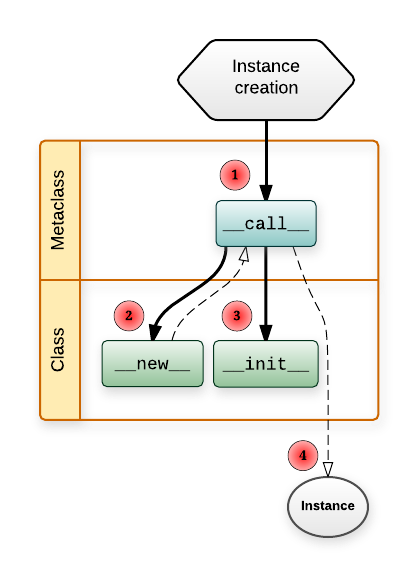
\includegraphics[width=0.7\onepicwidth]{figure/var/instance-creation}
        \caption{The diagram of how instances are constructed.\footnote{
                 \href{https://blog.ionelmc.ro/2015/02/09/understanding-python-metaclasses/}{Understanding Python metaclasses}}}
    \end{figure}
\end{frame}

\begin{frame}[fragile]
    \begin{tcblisting}{title=code snippe of tf 2.0 Variable}
            class VariableMetaclass(type):
              def _variable_v1_call(cls, **kwargs):
                pass

              def _variable_v2_call(cls, **kwargs):
                pass

              def __call__(cls, *args, **kwargs):
                if cls is VariableV1:
                  return cls._variable_v1_call(*args, **kwargs)
                elif cls is Variable:
                  return cls._variable_v2_call(*args, **kwargs)
                else:
                  return super(VariableMetaclass, cls).__call__(*args, **kwargs)

            @tf_export("Variable", v1=[])
            class Variable(six.with_metaclass(VariableMetaclass,
                                              checkpointable.CheckpointableBase)):
              def __init__(self, **kwargs):
                raise NotImplementedError
    \end{tcblisting}
    {\tiny \tt
    source: tensorflow/python/ops/variables.py \\[-2ex]
    commit: 4a5693e732b80a593bca7bf94ddd5df9e5d78cc0}
\end{frame}
